% Options for packages loaded elsewhere
\PassOptionsToPackage{unicode}{hyperref}
\PassOptionsToPackage{hyphens}{url}
%
\documentclass[
]{article}
\usepackage{amsmath,amssymb}
\usepackage{lmodern}
\usepackage{ifxetex,ifluatex}
\ifnum 0\ifxetex 1\fi\ifluatex 1\fi=0 % if pdftex
  \usepackage[T1]{fontenc}
  \usepackage[utf8]{inputenc}
  \usepackage{textcomp} % provide euro and other symbols
\else % if luatex or xetex
  \usepackage{unicode-math}
  \defaultfontfeatures{Scale=MatchLowercase}
  \defaultfontfeatures[\rmfamily]{Ligatures=TeX,Scale=1}
\fi
% Use upquote if available, for straight quotes in verbatim environments
\IfFileExists{upquote.sty}{\usepackage{upquote}}{}
\IfFileExists{microtype.sty}{% use microtype if available
  \usepackage[]{microtype}
  \UseMicrotypeSet[protrusion]{basicmath} % disable protrusion for tt fonts
}{}
\makeatletter
\@ifundefined{KOMAClassName}{% if non-KOMA class
  \IfFileExists{parskip.sty}{%
    \usepackage{parskip}
  }{% else
    \setlength{\parindent}{0pt}
    \setlength{\parskip}{6pt plus 2pt minus 1pt}}
}{% if KOMA class
  \KOMAoptions{parskip=half}}
\makeatother
\usepackage{xcolor}
\IfFileExists{xurl.sty}{\usepackage{xurl}}{} % add URL line breaks if available
\IfFileExists{bookmark.sty}{\usepackage{bookmark}}{\usepackage{hyperref}}
\hypersetup{
  hidelinks,
  pdfcreator={LaTeX via pandoc}}
\urlstyle{same} % disable monospaced font for URLs
\usepackage[margin=1in]{geometry}
\usepackage{color}
\usepackage{fancyvrb}
\newcommand{\VerbBar}{|}
\newcommand{\VERB}{\Verb[commandchars=\\\{\}]}
\DefineVerbatimEnvironment{Highlighting}{Verbatim}{commandchars=\\\{\}}
% Add ',fontsize=\small' for more characters per line
\usepackage{framed}
\definecolor{shadecolor}{RGB}{248,248,248}
\newenvironment{Shaded}{\begin{snugshade}}{\end{snugshade}}
\newcommand{\AlertTok}[1]{\textcolor[rgb]{0.94,0.16,0.16}{#1}}
\newcommand{\AnnotationTok}[1]{\textcolor[rgb]{0.56,0.35,0.01}{\textbf{\textit{#1}}}}
\newcommand{\AttributeTok}[1]{\textcolor[rgb]{0.77,0.63,0.00}{#1}}
\newcommand{\BaseNTok}[1]{\textcolor[rgb]{0.00,0.00,0.81}{#1}}
\newcommand{\BuiltInTok}[1]{#1}
\newcommand{\CharTok}[1]{\textcolor[rgb]{0.31,0.60,0.02}{#1}}
\newcommand{\CommentTok}[1]{\textcolor[rgb]{0.56,0.35,0.01}{\textit{#1}}}
\newcommand{\CommentVarTok}[1]{\textcolor[rgb]{0.56,0.35,0.01}{\textbf{\textit{#1}}}}
\newcommand{\ConstantTok}[1]{\textcolor[rgb]{0.00,0.00,0.00}{#1}}
\newcommand{\ControlFlowTok}[1]{\textcolor[rgb]{0.13,0.29,0.53}{\textbf{#1}}}
\newcommand{\DataTypeTok}[1]{\textcolor[rgb]{0.13,0.29,0.53}{#1}}
\newcommand{\DecValTok}[1]{\textcolor[rgb]{0.00,0.00,0.81}{#1}}
\newcommand{\DocumentationTok}[1]{\textcolor[rgb]{0.56,0.35,0.01}{\textbf{\textit{#1}}}}
\newcommand{\ErrorTok}[1]{\textcolor[rgb]{0.64,0.00,0.00}{\textbf{#1}}}
\newcommand{\ExtensionTok}[1]{#1}
\newcommand{\FloatTok}[1]{\textcolor[rgb]{0.00,0.00,0.81}{#1}}
\newcommand{\FunctionTok}[1]{\textcolor[rgb]{0.00,0.00,0.00}{#1}}
\newcommand{\ImportTok}[1]{#1}
\newcommand{\InformationTok}[1]{\textcolor[rgb]{0.56,0.35,0.01}{\textbf{\textit{#1}}}}
\newcommand{\KeywordTok}[1]{\textcolor[rgb]{0.13,0.29,0.53}{\textbf{#1}}}
\newcommand{\NormalTok}[1]{#1}
\newcommand{\OperatorTok}[1]{\textcolor[rgb]{0.81,0.36,0.00}{\textbf{#1}}}
\newcommand{\OtherTok}[1]{\textcolor[rgb]{0.56,0.35,0.01}{#1}}
\newcommand{\PreprocessorTok}[1]{\textcolor[rgb]{0.56,0.35,0.01}{\textit{#1}}}
\newcommand{\RegionMarkerTok}[1]{#1}
\newcommand{\SpecialCharTok}[1]{\textcolor[rgb]{0.00,0.00,0.00}{#1}}
\newcommand{\SpecialStringTok}[1]{\textcolor[rgb]{0.31,0.60,0.02}{#1}}
\newcommand{\StringTok}[1]{\textcolor[rgb]{0.31,0.60,0.02}{#1}}
\newcommand{\VariableTok}[1]{\textcolor[rgb]{0.00,0.00,0.00}{#1}}
\newcommand{\VerbatimStringTok}[1]{\textcolor[rgb]{0.31,0.60,0.02}{#1}}
\newcommand{\WarningTok}[1]{\textcolor[rgb]{0.56,0.35,0.01}{\textbf{\textit{#1}}}}
\usepackage{graphicx}
\makeatletter
\def\maxwidth{\ifdim\Gin@nat@width>\linewidth\linewidth\else\Gin@nat@width\fi}
\def\maxheight{\ifdim\Gin@nat@height>\textheight\textheight\else\Gin@nat@height\fi}
\makeatother
% Scale images if necessary, so that they will not overflow the page
% margins by default, and it is still possible to overwrite the defaults
% using explicit options in \includegraphics[width, height, ...]{}
\setkeys{Gin}{width=\maxwidth,height=\maxheight,keepaspectratio}
% Set default figure placement to htbp
\makeatletter
\def\fps@figure{htbp}
\makeatother
\setlength{\emergencystretch}{3em} % prevent overfull lines
\providecommand{\tightlist}{%
  \setlength{\itemsep}{0pt}\setlength{\parskip}{0pt}}
\setcounter{secnumdepth}{-\maxdimen} % remove section numbering
\ifluatex
  \usepackage{selnolig}  % disable illegal ligatures
\fi

\author{}
\date{\vspace{-2.5em}}

\begin{document}

\hypertarget{introactivity}{%
\section{Intro Skills Activity}\label{introactivity}}

\hypertarget{problem-1}{%
\subsection{Problem 1}\label{problem-1}}

\hypertarget{clear-enviro-rmlistls}{%
\section{clear enviro rm(list=ls())}\label{clear-enviro-rmlistls}}

Load the tidyverse and lubridate libraries.

library(tidyverse)

Read in the PINE\_NFDR\_Jan-Mar\_2010 csv using read\_csv()

Make a plot with the date on the x axis, discharge on the y axis. Show
the discharge of the two watersheds as a line, coloring by watershed
(StationID)

\begin{Shaded}
\begin{Highlighting}[]
\FunctionTok{library}\NormalTok{(tidyverse)}
\end{Highlighting}
\end{Shaded}

\begin{verbatim}
## -- Attaching packages --------------------------------------- tidyverse 1.3.1 --
\end{verbatim}

\begin{verbatim}
## v ggplot2 3.3.3     v purrr   0.3.4
## v tibble  3.1.2     v dplyr   1.0.6
## v tidyr   1.1.3     v stringr 1.4.0
## v readr   1.4.0     v forcats 0.5.1
\end{verbatim}

\begin{verbatim}
## -- Conflicts ------------------------------------------ tidyverse_conflicts() --
## x dplyr::filter() masks stats::filter()
## x dplyr::lag()    masks stats::lag()
\end{verbatim}

\begin{Shaded}
\begin{Highlighting}[]
\NormalTok{pine }\OtherTok{\textless{}{-}} \FunctionTok{read\_csv}\NormalTok{(}\StringTok{"PINE\_NFDR\_Jan{-}Mar\_2010.csv"}\NormalTok{)}
\end{Highlighting}
\end{Shaded}

\begin{verbatim}
## 
## -- Column specification --------------------------------------------------------
## cols(
##   StationID = col_character(),
##   cfs = col_double(),
##   surrogate = col_character(),
##   datetime = col_datetime(format = ""),
##   year = col_double(),
##   quarter = col_double(),
##   month = col_double(),
##   day = col_double()
## )
\end{verbatim}

\begin{Shaded}
\begin{Highlighting}[]
\FunctionTok{ggplot}\NormalTok{(pine, }\FunctionTok{aes}\NormalTok{(datetime, cfs, }\AttributeTok{color =}\NormalTok{ StationID))}\SpecialCharTok{+}
  \FunctionTok{geom\_line}\NormalTok{()}
\end{Highlighting}
\end{Shaded}

\includegraphics{03-Activity-Intro-Skills_files/figure-latex/unnamed-chunk-1-1.pdf}

\hypertarget{problem-2}{%
\subsection{Problem 2}\label{problem-2}}

Make a boxplot to compare the discharge of Pine to NFDR for February
2010.

Hint: use the pipe operator and the filter() function.

Hint2: when you filter dates, you have to let R know you're giving it a
date. You can do this by using the mdy() function from lubridate.

\begin{Shaded}
\begin{Highlighting}[]
\NormalTok{pine }\SpecialCharTok{\%\textgreater{}\%}
  \FunctionTok{filter}\NormalTok{(month }\SpecialCharTok{==} \DecValTok{2}\NormalTok{) }\SpecialCharTok{\%\textgreater{}\%}
  \FunctionTok{ggplot}\NormalTok{(}\FunctionTok{aes}\NormalTok{(StationID,cfs))}\SpecialCharTok{+}
  \FunctionTok{stat\_boxplot}\NormalTok{()}\SpecialCharTok{+}
  \FunctionTok{scale\_y\_log10}\NormalTok{()}
\end{Highlighting}
\end{Shaded}

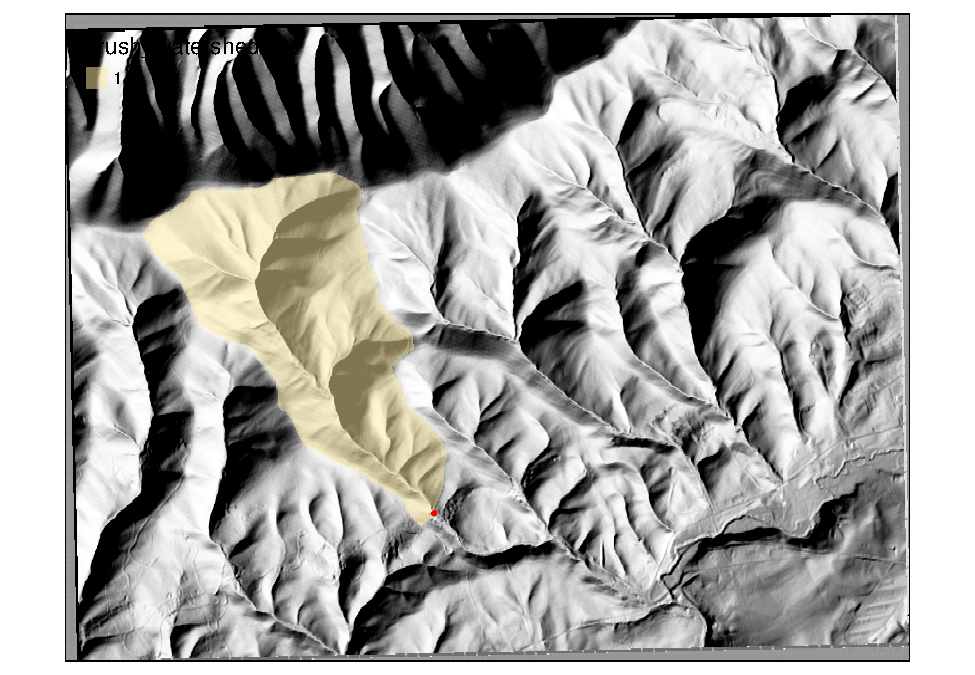
\includegraphics{03-Activity-Intro-Skills_files/figure-latex/unnamed-chunk-2-1.pdf}

\begin{Shaded}
\begin{Highlighting}[]
\CommentTok{\#pinefeb\textless{}{-} filter(pine,month == 2)}
\CommentTok{\#ggplot(pinefeb, aes(StationID,cfs))+}
  \CommentTok{\#stat\_boxplot()+}
  \CommentTok{\#scale\_y\_log10()}
\end{Highlighting}
\end{Shaded}

\hypertarget{problem-3}{%
\subsection{Problem 3}\label{problem-3}}

Read in the Flashy Dat Subset file.

For only sites in ME, NH, and VT: Plot PET (Potential
Evapotranspiration) on the X axis and RBI (flashiness index) on the Y
axis. Color the points based on what state they are in. Use the classic
ggplot theme.

\begin{Shaded}
\begin{Highlighting}[]
\NormalTok{flashy }\OtherTok{\textless{}{-}} \FunctionTok{read\_csv}\NormalTok{(}\StringTok{"Flashy\_Dat\_Subset.csv"}\NormalTok{)}
\end{Highlighting}
\end{Shaded}

\begin{verbatim}
## 
## -- Column specification --------------------------------------------------------
## cols(
##   .default = col_double(),
##   STANAME = col_character(),
##   STATE = col_character(),
##   CLASS = col_character(),
##   AGGECOREGION = col_character()
## )
## i Use `spec()` for the full column specifications.
\end{verbatim}

\begin{Shaded}
\begin{Highlighting}[]
\NormalTok{flashy }\SpecialCharTok{\%\textgreater{}\%}
  \FunctionTok{filter}\NormalTok{( STATE }\SpecialCharTok{\%in\%} \FunctionTok{c}\NormalTok{(}\StringTok{"ME"}\NormalTok{, }\StringTok{"NH"}\NormalTok{, }\StringTok{"VT"}\NormalTok{)) }\SpecialCharTok{\%\textgreater{}\%}
  \FunctionTok{ggplot}\NormalTok{(}\FunctionTok{aes}\NormalTok{(PET, RBI, }\AttributeTok{color =}\NormalTok{ STATE))}\SpecialCharTok{+}
  \FunctionTok{geom\_point}\NormalTok{() }\SpecialCharTok{+}
  \FunctionTok{theme\_classic}\NormalTok{()}
\end{Highlighting}
\end{Shaded}

\includegraphics{03-Activity-Intro-Skills_files/figure-latex/unnamed-chunk-3-1.pdf}

\hypertarget{problem-4}{%
\subsection{Problem 4}\label{problem-4}}

We want to look at the amount of snow for each site in the flashy
dataset. Problem is, we are only given the average amount of total
precip (PPTAVG\_BASIN) and the percentage of snow (SNOW\_PCT\_PRECIP).

Create a new column in the dataset called SNOW\_AVG\_BASIN and make it
equal to the average total precip times the percentage of snow (careful
with the percentage number).

Make a barplot showing the amount of snow for each site in Maine. Put
station name on the x axis and snow amount on the y. You have to add
something to geom\_bar() to use it for a 2 variable plot\ldots{} check
out the ggplot cheatsheet or do a quick internet search.

The x axis of the resulting plot looks terrible! Can you figure out how
to rotate the X axis labels so we can read them?

\begin{Shaded}
\begin{Highlighting}[]
\NormalTok{flashy }\SpecialCharTok{\%\textgreater{}\%}
  \FunctionTok{mutate}\NormalTok{(}\AttributeTok{SNOW\_AVG\_BASIN =}\NormalTok{ PPTAVG\_BASIN }\SpecialCharTok{*}\NormalTok{ SNOW\_PCT\_PRECIP }\SpecialCharTok{*} \FloatTok{0.01}\NormalTok{) }\SpecialCharTok{\%\textgreater{}\%}
  \FunctionTok{filter}\NormalTok{(STATE }\SpecialCharTok{==} \StringTok{"ME"}\NormalTok{) }\SpecialCharTok{\%\textgreater{}\%}
  \FunctionTok{ggplot}\NormalTok{(}\FunctionTok{aes}\NormalTok{(STANAME, SNOW\_AVG\_BASIN)) }\SpecialCharTok{+}
  \FunctionTok{geom\_bar}\NormalTok{(}\AttributeTok{stat=}\StringTok{"identity"}\NormalTok{,}\AttributeTok{position=}\StringTok{"dodge"}\NormalTok{)}\SpecialCharTok{+}
  \FunctionTok{coord\_flip}\NormalTok{()}
\end{Highlighting}
\end{Shaded}

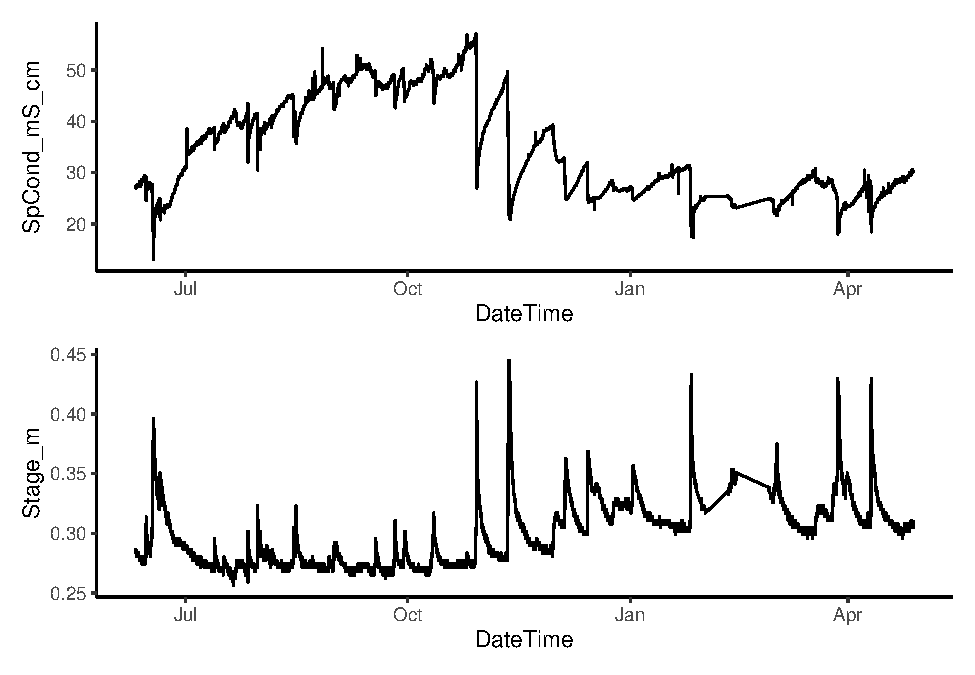
\includegraphics{03-Activity-Intro-Skills_files/figure-latex/unnamed-chunk-4-1.pdf}

\hypertarget{problem-5}{%
\subsection{Problem 5}\label{problem-5}}

Create a new tibble that contains the min, max, and mean PET for each
state. Sort the tibble by mean PET from high to low. Give your columns
meaningful names within the summarize function or using rename().

Be sure your code outputs the tibble.

\begin{Shaded}
\begin{Highlighting}[]
\NormalTok{flashyStatePET }\OtherTok{\textless{}{-}}\NormalTok{ flashy }\SpecialCharTok{\%\textgreater{}\%}
  \FunctionTok{group\_by}\NormalTok{(STATE) }\SpecialCharTok{\%\textgreater{}\%}
  \FunctionTok{summarize}\NormalTok{(}\AttributeTok{meanPET =} \FunctionTok{mean}\NormalTok{ (PET), }\AttributeTok{maxPET =} \FunctionTok{max}\NormalTok{(PET), }\AttributeTok{minPET =}\NormalTok{ (PET)) }\SpecialCharTok{\%\textgreater{}\%}
  \FunctionTok{arrange}\NormalTok{(meanPET)}
\end{Highlighting}
\end{Shaded}

\begin{verbatim}
## `summarise()` has grouped output by 'STATE'. You can override using the `.groups` argument.
\end{verbatim}

\hypertarget{problem-6}{%
\subsection{Problem 6}\label{problem-6}}

Take the tibble from problem 5. Create a new column that is the Range of
the PET (max PET - min PET). Then get rid of the max PET and min PET
columns so the tibble just has columns for State, mean PET, and PET
range.

Be sure your code outputs the tibble.

\begin{Shaded}
\begin{Highlighting}[]
\NormalTok{flashy\_range }\OtherTok{\textless{}{-}}\NormalTok{ flashyStatePET }\SpecialCharTok{\%\textgreater{}\%}
  \FunctionTok{mutate}\NormalTok{(}\AttributeTok{rangePET =}\NormalTok{ maxPET }\SpecialCharTok{{-}}\NormalTok{ minPET) }\SpecialCharTok{\%\textgreater{}\%}
  \FunctionTok{select}\NormalTok{(STATE, meanPET, rangePET)}
\end{Highlighting}
\end{Shaded}


\end{document}
